\documentclass[11pt, a4paper]{article}
\usepackage[a4paper, margin=2.5cm]{geometry}
% or, for US Letter paper instead of A4:
% \usepackage[letterpaper, margin=1in]{geometry}

\usepackage[utf8]{inputenc}
\usepackage[T1]{fontenc}
\usepackage[english]{babel}
\usepackage{amsmath}
\usepackage{amsfonts}
\usepackage{amssymb}
\usepackage{amsmath, amssymb}   % for equations, matrices, etc.
\usepackage{graphicx}           % for figures
\usepackage{hyperref}           % for clickable links/citations\usepackage[font=scriptsize]{caption}
\usepackage{parskip}
\usepackage{titling}
\usepackage{subcaption}
\usepackage{float}
\usepackage{placeins}
\usepackage{graphicx}
\usepackage{tikz}
\captionsetup{font=footnotesize}


\usepackage[numbers]{natbib}
\numberwithin{equation}{section}
\definecolor{aicolor}{HTML}{6E2A8C}
\ifdefined\hideai
  \long\def\ai#1{}
  \long\def\aicorrection#1#2{#1}
\else
  \long\def\ai#1{{\color{aicolor}#1}}
  \long\def\aicorrection#1#2{\ai{#2}}
\fi

\title{Advanced Seminar: Specialized Topics in Theoretical Physics \\[1ex] \large \textbf{Bulk Topology in the Kitaev Chain}}
\author{Schewtschik, Guilherme (3748052)}
\date{\today}

\begin{document}
\maketitle

\abstract{This report summarizes the first block of the Advanced Seminar course quantum project. It discusses the foundations of the Kitaev chain and explains how bulk topology arises in this context. The report introduces the concept of Majorana fermions, discusses the Kitaev Hamiltonian, and presents the winding number as a topological invariant that distinguishes the trivial and topological phases of the system.}


\section{Introduction}

First described by \textit{Alexei Yu. Kitaev} in his 2000 paper~\cite{Kitaev2000}, the Kitaev chain is a toy model used to study topological superconductors and topological quantum computing. It builds upon the work of the Italian physicist \textit{Ettore Majorana}, whose concept of Majorana fermions gives rise to localized edge modes that provide a promising platform for topologically protected quantum computation.

The Kitaev chain exhibits a topological phase transition and serves as an ideal framework for understanding the relationship between superconductivity, Majorana edge states, and bulk topology. In particular, it demonstrates how a system's topological properties can be characterized by bulk invariants and how these invariants determine the existence of robust edge states through the bulk-boundary correspondence.



\section{Majorana Fermions}\label{sec:Majorana}
\aicorrection
{Majorana fermions are a theoretical fermionic particle with the special property of being their own antiparticle, first proposed by \textit{Ettore Majorana} in his 1937 paper \textit{''A symmetric theory of electrons and positrons''}~\cite{Majorana1937}, where he describes chargeless spin=$\frac{1}{2}$ particles with real spinor fields.}
{Majorana fermions are theoretical fermionic particles with the special property of being their own antiparticles. They were first proposed by \textit{Ettore Majorana} in his 1937 paper \textit{A Symmetric Theory of Electrons and Positrons}~\cite{Majorana1937}, in which he describes chargeless spin-$\frac{1}{2}$ particles with real spinor fields.}

\aicorrection
{In a field theoretical perspective we describe fermions with the so called fermionic annihilation and creation operators, denoted by $a(\mathbf{k}),a^\dagger(\mathbf{k})$ for particles and by $b(\mathbf{k}),b^\dagger(\mathbf{k})$ for anti-particles, such that their wave function is given by~\cite{Srednicki2007}:}
{From a field-theoretical perspective, we describe fermions using the so-called annihilation and creation operators $a(\mathbf{k}),a^\dagger(\mathbf{k})$ for particles and $b(\mathbf{k}),b^\dagger(\mathbf{k})$ for antiparticles. Their wave function is~\cite{Srednicki2007}:}
\begin{equation}
    \psi(x) = \sum_{s} \int \frac{d^3k}{(2 \pi )^3 2\omega(\mathbf{k})} \left( a(\mathbf{k})u_s e^{ikx} + b^\dagger(\mathbf{k}) v_s e^{-ikx}\right)
    \label{eq:canonical_quantization_fermion}
\end{equation}

\aicorrection
{Since Majorana fermions are their own anti particle we can set $b(\mathbf{k}) = a(\mathbf{k})$; furthermore, charge conjugation imposes $u_s^* = v_s$~\cite{Srednicki2007}, so we can rewrite the wave function as:}
{Because Majorana fermions are their own antiparticles, we can set $b(\mathbf{k})=a(\mathbf{k})$. Furthermore, charge conjugation imposes $u_s^*=v_s$~\cite{Srednicki2007}, so the wave function becomes}

\begin{equation}
    \psi(x) = \sum_{s} \int \frac{d^3k}{(2 \pi )^3 2\omega(\mathbf{k})} \left( a(\mathbf{k})u_s e^{ikx} + a^\dagger(\mathbf{k}) u_s^* e^{-ikx}\right)
\end{equation}

Now expanding the exponential terms we can write the wave function as:

\begin{equation}
    \psi(x) = \sum_{s} \int \frac{d^3k}{(2 \pi )^3 2\omega(\mathbf{k})} \left( (a(\mathbf{k})u_s + a^\dagger(\mathbf{k})u_s^*)\cos(kx) + i(a(\mathbf{k})u_s - a^\dagger(\mathbf{k})u_s^*)\sin(kx)\right)
\end{equation}

\aicorrection{So we difine the operators $c_A$ and $c_B$ as follows:}{We group the cosine and sine coefficients into the spinor-valued combinations}

\begin{equation}
    \aicorrection{c_{A,s}=a(\mathbf{k})u_s+a^\dagger(\mathbf{k})u_s^*,\quad c_{B,s}=i(a(\mathbf{k})u_s-a^\dagger(\mathbf{k})u_s^*)}{\mathcal{C}_{A,s}(\mathbf{k})=a(\mathbf{k})u_s+a^\dagger(\mathbf{k})u_s^*,\quad \mathcal{C}_{B,s}(\mathbf{k})=i\left[a(\mathbf{k})u_s-a^\dagger(\mathbf{k})u_s^*\right]}
\end{equation}

\aicorrection{This is the most general form of the Majorana operators, we can pin a representation by choosing our spinor basis:}{For example, one may choose the following explicit spinor basis:}

\[
\aicorrection{u_\uparrow=\begin{pmatrix}1\\0\\1\\0\end{pmatrix},\quad u_\downarrow=\begin{pmatrix}0\\1\\0\\1\end{pmatrix}}{u_\uparrow=\begin{pmatrix}1\\0\\1\\0\end{pmatrix},\qquad u_\downarrow=\begin{pmatrix}0\\1\\0\\1\end{pmatrix}}
\]

\aicorrection{In this special case the form is independent of the spin index $s$, so we retrieve the representation used in Kitaev's original paper~\cite{Kitaev2000}:}{These continuum spinors are distinct from the scalar lattice Majorana operators. For the spinless Kitaev chain, define the site-local Hermitian operators instead:}

\begin{equation}
    \aicorrection{c_A=a(\mathbf{k})+a^\dagger(\mathbf{k}),\quad c_B=i(a(\mathbf{k})-a^\dagger(\mathbf{k}))}{\gamma_{A,j}=a_j+a_j^\dagger,\quad \gamma_{B,j}=i(a_j-a_j^\dagger)}
\end{equation}

\aicorrection
{One physical interpretation of the Majorana fermion is that the original fermion can be ''split'' into two Majorana fermions in the same physical position but at different ''Majorana sites''~\cite{Kitaev2000}, this is going to be of extreme importance when building the Kitaev chain in the next section.}
{One physical interpretation is that an ordinary fermion can be split into two Majorana fermions at the same physical position but on different Majorana sites~\cite{Kitaev2000}. This picture is important when constructing the Kitaev chain in the next section.}

\aicorrection{It is also practical for the future to write our fermionic operators in terms of our Majorana operators:}{For later use, it is convenient to express the fermionic operators in terms of the Majorana operators:}

\begin{equation}
    \aicorrection{a(\mathbf{k})=\frac{c_A-ic_B}{2},\quad a^\dagger(\mathbf{k})=\frac{c_A+ic_B}{2}}{a_j=\frac{\gamma_{A,j}-i\gamma_{B,j}}{2},\quad a_j^\dagger=\frac{\gamma_{A,j}+i\gamma_{B,j}}{2}}
\end{equation}




\section{Kitaev Hamiltonian}\label{sec:Kitaev}
\aicorrection
{To construct our Hamiltonian, we first define the physical system. Kitaev considers a chain of spin aligned electrons on a p-wave superconductor~\cite{Kitaev2000}. This allows triplet like pairing at adjacent sites. Furthermore, electrons can be absorbed or released in Cooper pairs, so parity, rather than particle number, is preserved.}
{To construct the Hamiltonian, we first define the physical system. Kitaev considers a chain of spin-aligned electrons coupled to a p-wave superconductor~\cite{Kitaev2000}. This allows triplet-like pairing between adjacent sites. Furthermore, electrons can enter or leave in Cooper pairs, so fermion parity, rather than particle number, is conserved.}

\aicorrection{With this taken into consideration Kitaev introduces our system's Hamiltonian~\cite{Kitaev2000}:}{With these considerations in mind, Kitaev introduces the system's Hamiltonian~\cite{Kitaev2000}:}
\begin{equation}
    \aicorrection
    {H = \sum_j -w(a^\dagger_{j}a_{j+1} + a^\dagger_{j+1}a_j)-\mu(a^\dagger_j a_j - \frac{1}{2})+\Delta a_{j}a_{j+1} + \Delta^*a^\dagger_{j+1}a^\dagger_{j}}
    {H = -w\sum_{j=1}^{L-1}(a_j^\dagger a_{j+1}+a_{j+1}^\dagger a_j)-\mu\sum_{j=1}^{L}(a_j^\dagger a_j-\frac12)+\sum_{j=1}^{L-1}(\Delta a_j a_{j+1}+\Delta^*a_{j+1}^\dagger a_j^\dagger)}
    \label{eq:kitaev_Hamiltonian_fermi}
\end{equation}


\aicorrection
{Here we anotate the fermionic operators at site $j$ by $a_j$, where $j \in [1,L]$ is the chain position index. The constants $w,\mu$, and $\Delta$ correspond to hopping, chemical potential, and superconducting pairing.}
{Here, $a_j$ and $a_j^\dagger$ denote the annihilation and creation operators at site $j$, where $j=1,\ldots,L$. The constants $w$, $\mu$, and $\Delta$ describe hopping, the chemical potential, and superconducting pairing, respectively.}

As $\Delta$ is in general a complex number $\Delta = |\Delta|e^{i\theta}$, we can incorporate this phase factor into our definition of the Majorana Fermions, with this we may express the Hamiltonian in the following way~\cite{Kitaev2000}:
\begin{equation}
    \aicorrection
    {H = \frac{i}{2}\sum_j -\mu c_{B,j}c_{A,j}+(w+|\Delta|)c_{B,j}c_{A,j+1}+(-w+|\Delta|)c_{B,j+1}c_{A,j}}
    {H = \frac{i}{2}\left[-\mu\sum_{j=1}^{L}c_{B,j}c_{A,j}+\sum_{j=1}^{L-1}\left((w+|\Delta|)c_{B,j}c_{A,j+1}+(|\Delta|-w)c_{B,j+1}c_{A,j}\right)\right]}
    \label{eq:kitaev_Hamiltonian_Majorana}
\end{equation}



\aicorrection{The chemical potential term pairs Majorana fermions at the same site, while the terms depending on $w$ and $|\Delta|$ pair them at different sites.}{The chemical-potential term pairs Majorana fermions at the same site, whereas the terms proportional to $w$ and $|\Delta|$ pair them at different sites. This distinction allows unpaired Majorana fermions to appear at the chain ends.}

\aicorrection{Taking $w$ and $|\Delta|$ to zero gives the Trivial mode, where the chemical potential survives and the Majorana fermions remain localized.}{Setting $w=|\Delta|=0$ gives the trivial limit, where only the chemical-potential term survives and the Majorana fermions remain paired locally.}

\begin{figure}[h]
\centering
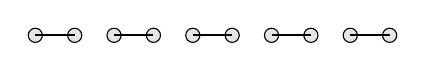
\begin{tikzpicture}[scale=0.5]
    \foreach \x in {0,1,2,3,4,5,6,7,8,9}
    {
      \draw[fill=gray!20] (\x,0) circle (0.18);
    }
    \draw[thick] (0,0)--(1,0);
    \draw[thick] (2,0)--(3,0);
    \draw[thick] (4,0)--(5,0);
    \draw[thick] (6,0)--(7,0);
    \draw[thick] (8,0)--(9,0);
\end{tikzpicture}
\caption{\small Majorana pairing pattern along the Kitaev chain in the trivial mode.}
\label{fig:kitaev-chain-trivial}
\end{figure}

\aicorrection{The Topological Mode occurs when $|\Delta| = w > 0, \mu = 0$, where our Hamiltonian becomes:}{The topological limit occurs for $|\Delta|=w>0$ and $\mu=0$, where the Hamiltonian becomes}
\begin{equation}
    \aicorrection{H = iw \sum c_{B,j}c_{A,j+1}}{H = iw\sum_{j=1}^{L-1}c_{B,j}c_{A,j+1}}
    \label{eq:kitaev_Hamiltonian_topological}
\end{equation}
\aicorrection{Now the Majorana fermions pair with the adjacent spatial site, and we get unpaired fermions at $c_{A,1}$ and $c_{B,L}$}{The Majorana fermions now pair across adjacent sites, leaving $c_{A,1}$ and $c_{B,L}$ unpaired.}

\begin{figure}[h]
\centering
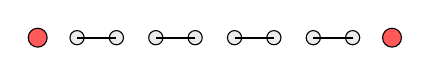
\begin{tikzpicture}[scale=0.5]
    \foreach \x in {0,1,2,3,4,5,6,7,8}{\draw[fill=gray!15] (\x,0) circle (0.18);}
      \draw[thick] (1,0)--(2,0);
      \draw[thick] (3,0)--(4,0);
      \draw[thick] (5,0)--(6,0);
      \draw[thick] (7,0)--(8,0);
      \draw[fill=red!65] (0,0) circle (0.24);
      \draw[fill=red!65] (9,0) circle (0.24);
      %\draw[dashed,thick,red!70] (0.2,0.35) .. controls (4.5,0.9) .. (8.8,0.35);
\end{tikzpicture}
\caption{\small Majorana pairing pattern along the Kitaev chain in the topological mode}
\label{fig:kitaev-chain-topological}
\end{figure}

% We can thus define a new fermionic operator from our Majorana fermions~\cite{Kitaev2000}:

% \begin{equation}
%     \tilde{a}_j=\frac{1}{2}(c_{B,j} + ic_{A,j+1}), \quad \tilde{a}_j^\dagger=\frac{1}{2}(c_{B,j} - ic_{A,j+1})
% \end{equation}

% Getting the new Hamiltonian:

% \begin{equation}
%     H = 2w\sum \left(\tilde{a_j}^\dagger\tilde{a_j} + \frac{1}{2}\right)
% \end{equation}

% The ground state gets annihilated by the operator $\tilde{a}_j$, but the states at the edges dont get annihlated, so acting with
% $c_{A,1}$ and $c_{B,2}$ on the ground state $|\psi_0\langle$ leaves it unchanged

\aicorrection{The topological phase is not restricted to $|\Delta|=w>0,\mu=0$; in the thermodynamical limit it also exists for $\Delta\neq0$ and $|\mu|<2w$~\cite{Herviou2017}.}{The topological phase is not restricted to $|\Delta|=w>0$ and $\mu=0$. In the thermodynamic limit, it persists for $\Delta\neq0$ and $|\mu|<2w$~\cite{Herviou2017}. Section~\ref{sec:Topology} discusses this regime in more detail.}

\aicorrection{To continue the analysis of our Hamiltonian it is advantageous to take our fermionic operators into momentum space, and work in the reciprocal space from now on:}{To continue the analysis, it is convenient to transform the fermionic operators to momentum space:}
\begin{equation}
    \aicorrection
    {a_k = \frac{1}{\sqrt{L}}\sum a_j e^{ikj}, \quad a_k^\dagger = \frac{1}{\sqrt{L}}\sum a_j e^{-ikj}}
    {a_j = \frac{1}{\sqrt L}\sum_{k\in\mathrm{BZ}}e^{ikj}a_k,\quad a_j^\dagger = \frac{1}{\sqrt L}\sum_{k\in\mathrm{BZ}}e^{-ikj}a_k^\dagger}
    \label{eq:operators_momentum_space}
\end{equation}

\aicorrection{With this our Hamiltonian in momentum space is:}{With this transformation, the momentum-space Hamiltonian is}
\begin{equation}
    \aicorrection
    {H_k = \sum (-\mu - 2w\cos(k))a_k^\dagger a_k + i\Delta\sin(k)(a_k^\dagger a_{-k}^\dagger-a_{-k}a_k)}
    {H = \sum_{k\in\mathrm{BZ}}\left[\xi_k a_k^\dagger a_k+i\Delta\sin k\left(a_k^\dagger a_{-k}^\dagger-a_{-k}a_k\right)\right],\quad \xi_k=-\mu-2w\cos k}
    \label{eq:Hamiltonian_momentum_space}
\end{equation}

\aicorrection{We can also write our Hamiltonian as:}{Pairing $k$ with $-k$, the Hamiltonian becomes a sum of BdG blocks:}
\begin{equation}
    \aicorrection{H_k = \sum \Psi_k^\dagger h(k)\Psi_k}{H = \sum_{k>0}\Psi_k^\dagger h(k)\Psi_k}
\end{equation}

\aicorrection{Where $h(k)$ is a $2\times2$ Matrix and $\Psi_k$ is the Nambu vector:}{Here, $h(k)$ is a $2\times2$ matrix and $\Psi_k$ is the Nambu spinor}
\[
\Psi_k = \begin{pmatrix} a_k \\ a^\dagger_{-k} \end{pmatrix}
\]

\aicorrection{So our matrix $h(k)$ is explicitly:}{The matrix $h(k)$ is explicitly}
\[
h(k) = \begin{pmatrix}          \xi_k & 2i\Delta\sin(k)\\
                        -2i\Delta\sin(k)& -\xi_k \end{pmatrix}
\]

\aicorrection{Where $\xi_k=-\mu-2w\cos k$, the Hamiltonian's spectrum is:}{The two BdG branches are}
\begin{equation}
    \aicorrection{E_k = \sqrt{(\mu+2w\cos k)^2+(2\Delta\sin k)^2}}{E_\pm(k)=\pm\sqrt{(-\mu-2w\cos k)^2+(-2\Delta\sin k)^2}}
    \label{eq:energy_kitaev_chain}
\end{equation}

\aicorrection
{The energy differs between the phases, and the gap closes at the critical point. At $k=0$, $E_0=|2w+\mu|$, while at $k=\pi$, $E_\pi=|2w-\mu|$.}
{Figure~\ref{fig:bulk_dispersion} shows how the spectrum differs between the two phases. At $k=0$, $E_0=|2w+\mu|$, while at $k=\pi$, $E_\pi=|2w-\mu|$. The gap therefore closes at $\mu=\pm2w$.}

\begin{figure}[ht]
    \centering
    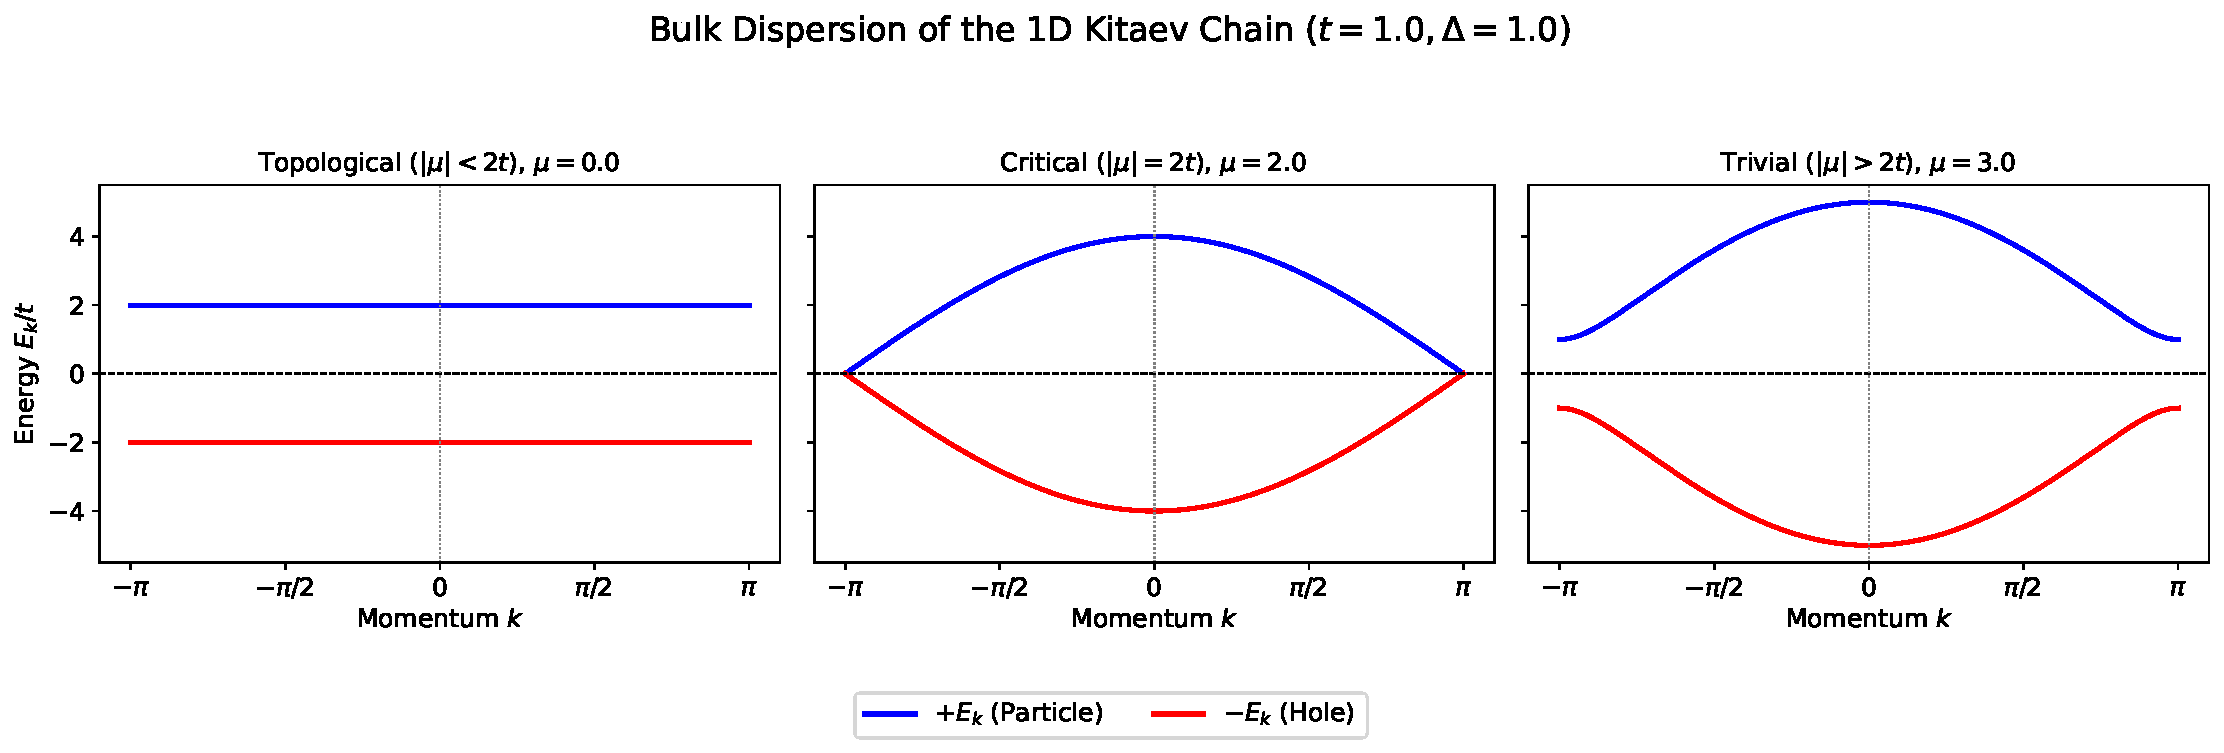
\includegraphics[width=0.8\linewidth]{../../plots/block1_07_bulk_dispersion_panels.pdf}
    \caption{\aicorrection{Bulk energy dispersion for different values of $\mu$ and $w$, ($t=w$).}{Bulk energy dispersion for different values of $\mu$ and $w$ ($t=w$).}}
    \label{fig:bulk_dispersion}
\end{figure}

\newpage

\aicorrection
{This gives us an idea of where the transition occurs, but we need a parameter solely dependent on topology.}
{This spectrum indicates where the transition occurs. To characterize the topology directly, however, we need a quantity that depends only on the system's topological structure: the winding number.}

\section{Topology}\label{sec:Topology}

\aicorrection{To construct the winding number first we rewrite the matrix $h(k)$ in terms of the Pauli matrices:}{To construct the winding number, we first express $h(k)$ in terms of Pauli matrices:}

\begin{equation}
    h(k) = -(\mu + 2w\cos(k)) \sigma_z - 2|\Delta|\sin(k)\sigma_y
\end{equation}

\aicorrection{We define $\mathbf{n}(k)$ to visualise the topology and plot it in figure~\ref{fig:vector_n}.}{We define $\mathbf{n}(k)=-(2|\Delta|\sin k,\mu+2w\cos k)$ to visualize the topology. Figure~\ref{fig:vector_n} shows its trajectory.}

\begin{figure}[ht]
    \centering
    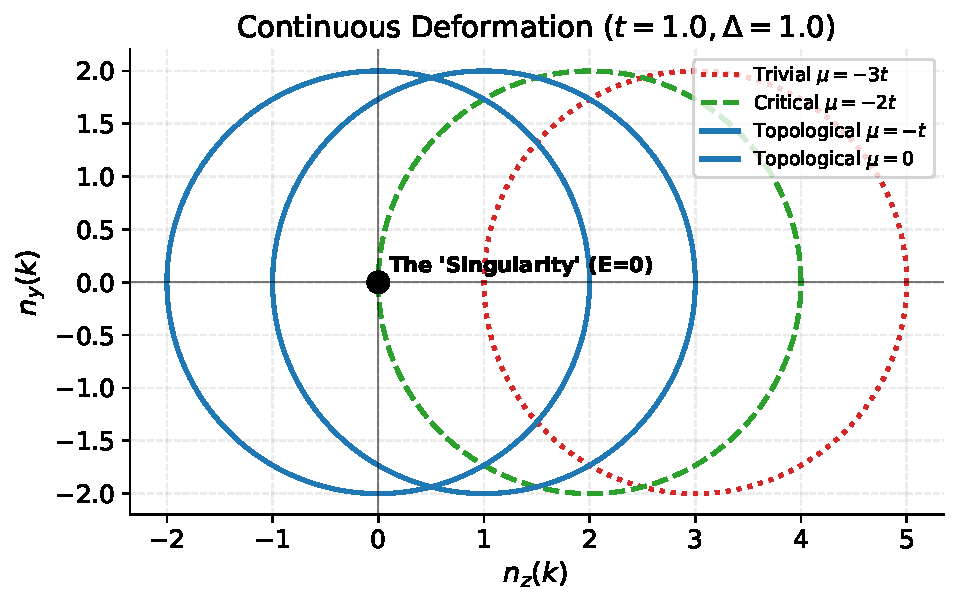
\includegraphics[width=0.5\linewidth]{../../plots/block1_02_trajectory_deformation.pdf}
    \caption{$\mathbf{n}(k)$ for different values of $\mu$ and $w$, ($t=w$).}
    \label{fig:vector_n}
\end{figure}

\aicorrection{The topological curve encircles the origin, the trivial curve does not, and the critical curve touches it.}{In the topological phase, the trajectory encircles the origin; in the trivial phase, it does not. At the critical point, the curve touches the origin. More rigorously, the winding number is}

\begin{equation}
    \nu =  \int \frac{d\theta_k}{dk}\frac{dk}{2\pi}
\end{equation}

Where $\theta_k$ is:
\begin{equation}
    \aicorrection{\theta_k=\arg((\mu+2w\cos k)+i(2|\Delta|\sin k))}{\theta_k=\arg\!\left[n_z(k)+i n_y(k)\right]=\arg\!\left[-\mu-2w\cos k-i2|\Delta|\sin k\right]}
\end{equation}

\aicorrection{This tells us whether a configuration is trivial or topological by whether the curve encompasses the origin.}{The winding number determines whether a parameter set is trivial or topological by recording whether the curve encircles the origin.}

\begin{figure}[ht]
    \centering
    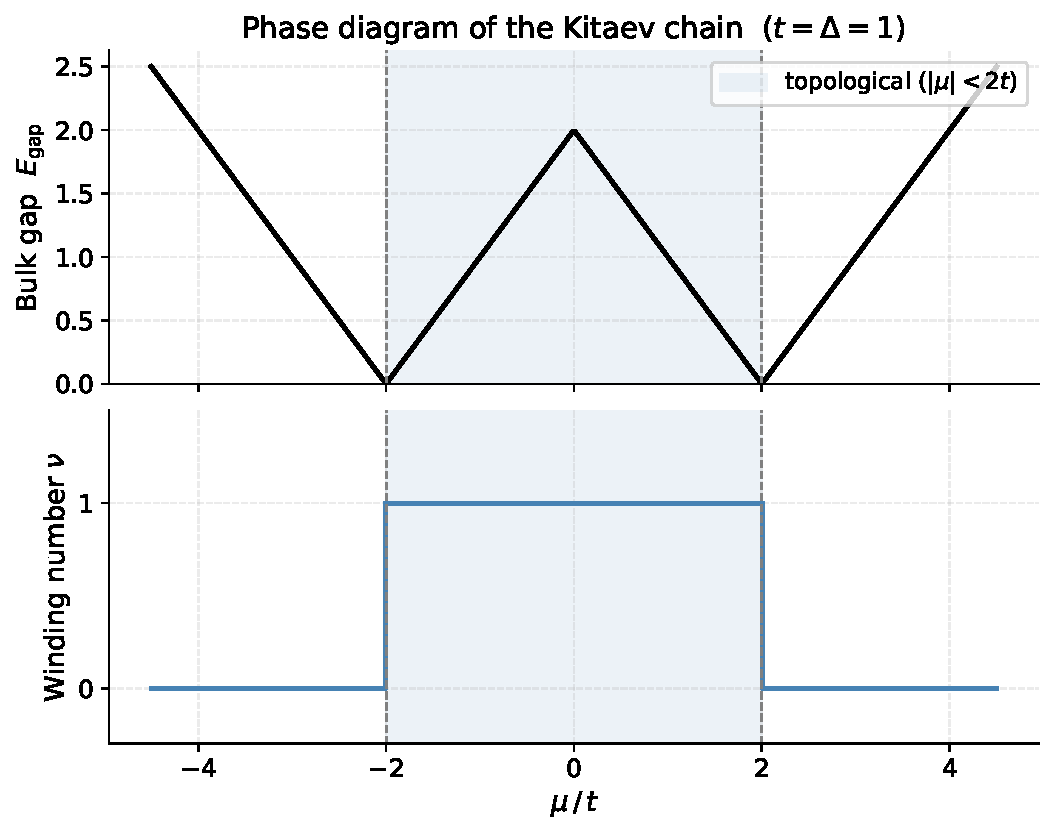
\includegraphics[width=0.5\linewidth]{../../plots/block1_03_phase_diagram.pdf}
    \caption{$\nu$ for different values of $\mu$ and $w$, alongside the Bulk energy gap, ($t=w$).}
    \label{fig:phase_diagram}
\end{figure}

\section{Conclusion}

The Kitaev chain provides one of the simplest models for studying topological superconductivity and the emergence of Majorana edge modes. Depending on the values of the system parameters, the chain can exist in either a trivial or a topological phase. The transition between these phases occurs only when the bulk energy gap closes, highlighting the intimate connection between the bulk spectrum and the existence of edge states.

The topological properties of the system can be characterized by the winding number, a bulk topological invariant that distinguishes the two phases by describing the behavior of the Hamiltonian in momentum space. This provides a clear and intuitive framework for identifying the topology of the system without directly examining its edge states, illustrating the principle of bulk-boundary correspondence.

Although the Kitaev chain is an idealized model, it captures the essential physics of one-dimensional topological superconductors and serves as a fundamental example in the study of topological phases of matter.
\subsection{Large Language Models as a Tool for Physics Research}

Throughout this course, one of our objectives was to evaluate and analyze how large language models (LLMs) can be integrated into physics research and the broader process of learning and scientific understanding.

In my experience, LLMs are a double-edged sword. On one hand, when used appropriately, they can significantly accelerate the learning process by gathering relevant resources, locating articles and reference material, and assisting with repetitive or time-consuming tasks. During this course, they proved particularly useful for compiling reports, preparing presentation slides, and supporting the implementation of code for the numerical simulations carried out in the later stages of the project.

On the other hand, excessive reliance on LLMs may lead to a false sense of understanding, as they can provide convincing explanations without encouraging the user to critically engage with the underlying concepts. They may also discourage the independent reasoning and analytical thinking that are essential when conducting scientific research. For this reason, I believe that LLMs should be regarded as tools that complement, rather than replace, traditional learning methods and critical thinking.

\subsection{Acknowledgments}

\aicorrection{The notation differs from the course slides because I followed Kitaev's original paper~\cite{Kitaev2000}. The use of LLMs was limited to grammar correction and locating references.}{The notation differs from that used in the course slides because I predominantly followed Kitaev's original paper~\cite{Kitaev2000}. Large language models were used only for grammar correction and assistance in locating references.}

\newpage
\bibliographystyle{plainnat}
\bibliography{references}

\end{document}
